\section{Characterization and Automated Detection of Insect Chemosensory Receptors}

\subsection{Introduction}

\subsection{Methods}

\subsubsection{Characterization}

\subsubsection{Identification Approach 1: Digrams, Weighting, and Clustering}

\subsubsection{Identification Approach 2: Profile Hidden Markov Models (HMMs)}

\begin{figure}[H]
  \centering
  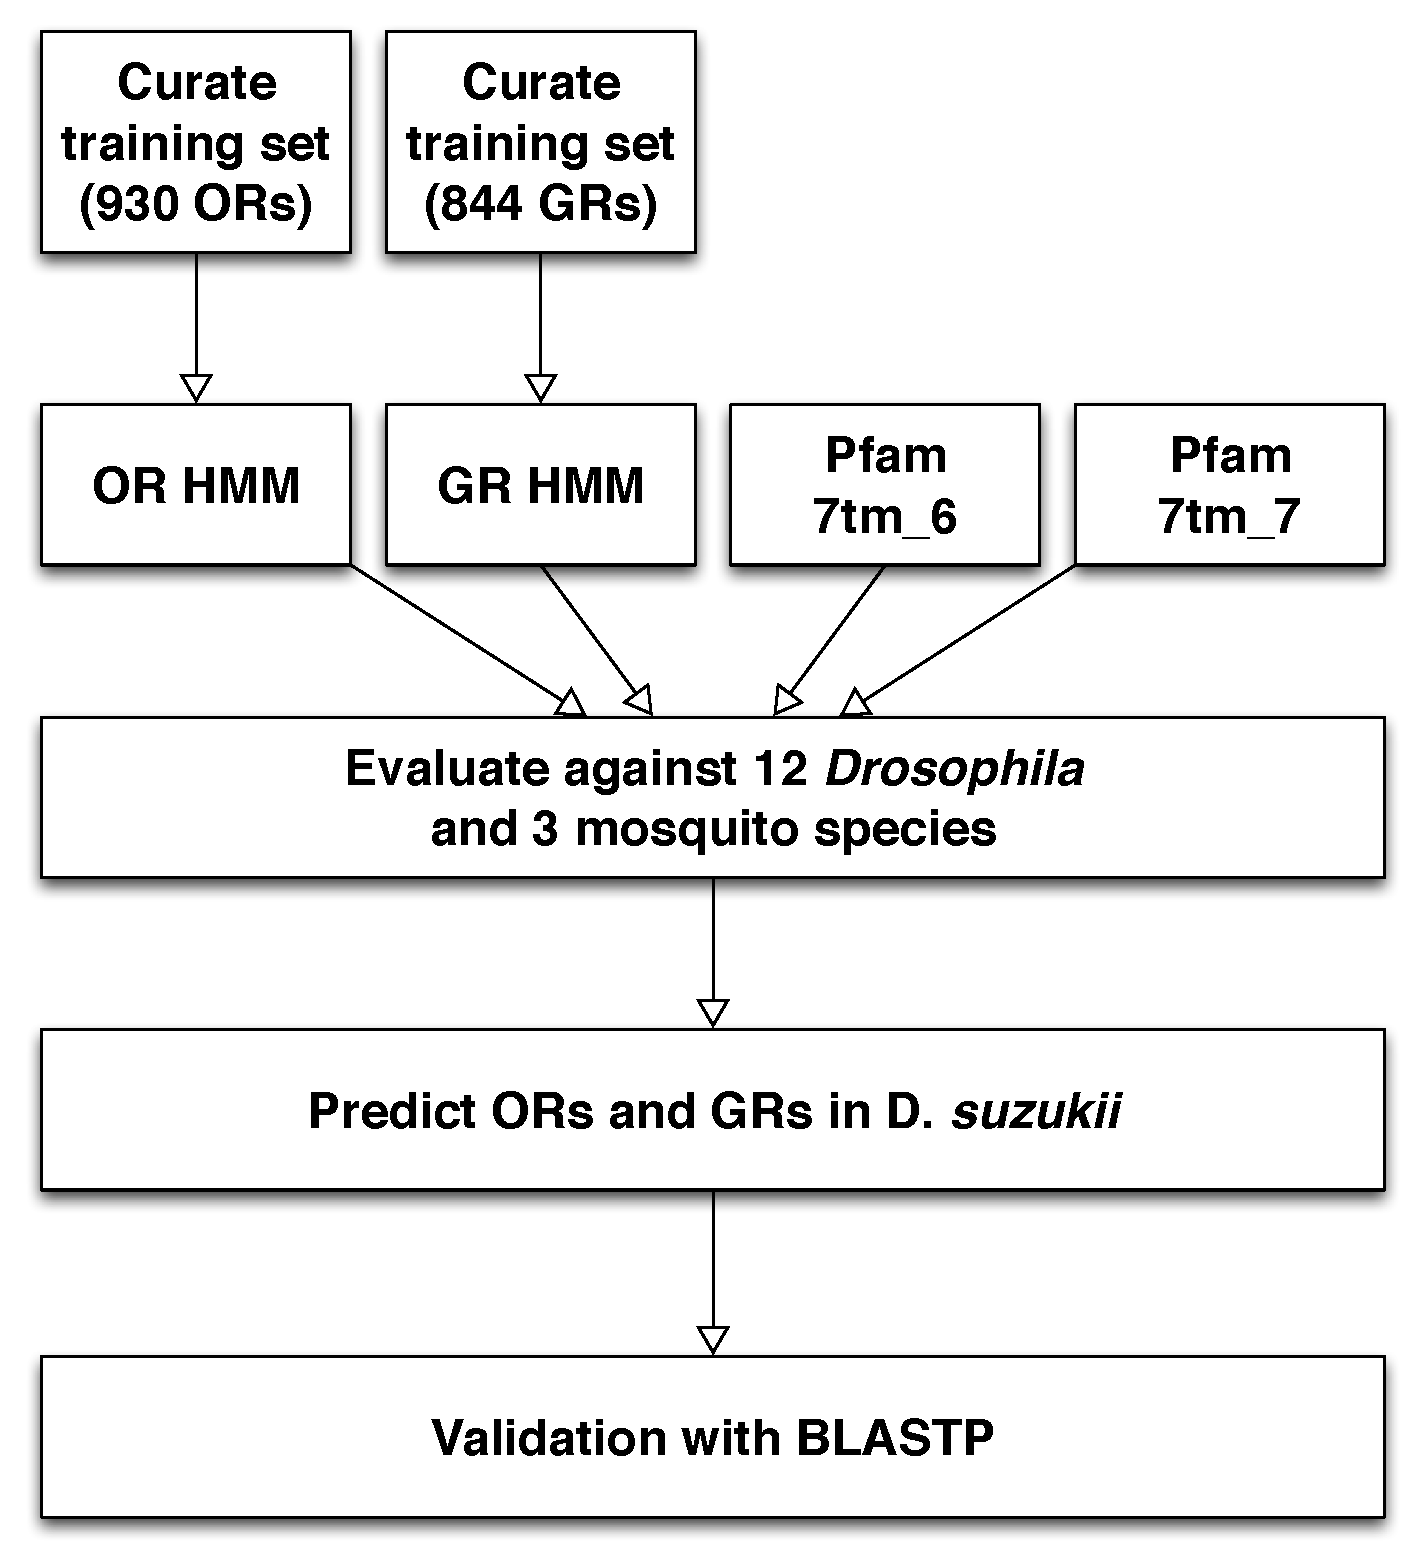
\includegraphics[width=0.7\textwidth]{figures/chemosensory/hmm_workflow}
  \caption{Workflow for HMM training, validation, and classification}
  \label{fig:chemosensory:hmm-workflow}
\end{figure}

\subsection{Results}

\subsubsection{Characterization of Insect Chemosensory Receptors}

\begin{figure}[H]
  \centering
  \begin{subfigure}[b]{0.45\textwidth}
    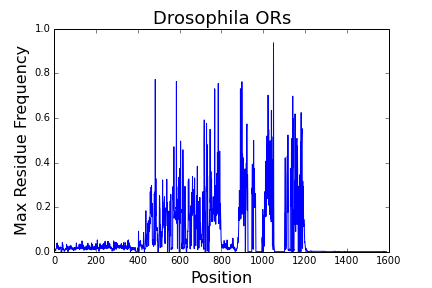
\includegraphics[width=\textwidth]{figures/chemosensory/drosophila_or_max_freq.png}
    \caption{Olfactory Receptors (930)}
    \label{fig:chemosensory:or-max-freq}
  \end{subfigure}
  ~
  \begin{subfigure}[b]{0.45\textwidth}
    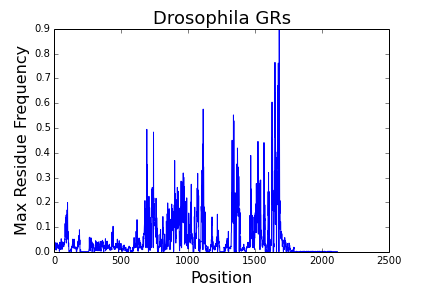
\includegraphics[width=\textwidth]{figures/chemosensory/drosophila_gr_max_freq.png}
    \caption{Gustatory Receptors (844)}
    \label{fig:chemosensory:gr-max-freq}
  \end{subfigure}
\label{fig:chemosensory:max-freq}
\caption{}
\end{figure}

\subsubsection{Comparing Approaches for Automated Identification}

\begin{table}[H]
  \centering
  \begin{tabular}{c c c c} \hline
  \emph{HMM} & \emph{Olfactory Receptors} & \emph{Gustatory Receptors} & \emph{Others} \\ \hline
  7tm\_6 & 881 & 15 & 223 \\ \hline
  OR & 928 & 68 & 297 \\ \hline
  7tm\_7 & 213 & 829 & 580 \\ \hline
  GR & 131 & 828 & 271 \\ \hline
  \end{tabular}
  \caption{Predicted Proteins from 12 \textit{Drosophila} and 3 mosquito species}
  \label{tab:chemosensory:hmm-validation}
\end{table}

\subsubsection{Identification of \emph{D. suzukii} Chemosensory Receptors}

\subsubsection{validation of \emph{D. suzukii} Chemosensory Receptors}

\subsection{Discussion and Conclusion}